\chapter{Theoretische Einführung}
\label{chapter:theo}

\section{Theoretische Grundlagen der NMR} \label{section:theo:grundlagen}


Ziel der NMR ist es, Kernspins einer Probe zu manipulieren und zu beobachten.
Da Spins $I$ über
\begin{align}
    \vec{\mu} = \gamma \hbar \vec{I}
\end{align}
mit magnetischen Dipolen $\mu$ verknüpft sind, ist die Beeinflussung von Spins mithilfe von Magnetfeldern möglich. Der Proportionalitätsfaktor $\gamma$ ist als gyromagnetisches Verhältnis bekannt und eine isotopenabhängige Konstante.

Werden die Kernspins einem Magnetfeld $\vec{B}_0 = (0, 0, B_{0,z})$ ausgesetzt, spalten die Energiezustände nach Zeeman auf. Die potentielle Energie eines magnetischen Dipols ist $E = - \vec{\mu} \vec{B}_0$. Mit obigen Beziehungen resultiert demnach $E = - \gamma \hbar I_z B_{0,z}$. Die Eigenwerte von $I_z$ lauten $m = -I, -I + 1, \dots, I - 1, I$; somit ist die Energiedifferenz zwischen zwei benachbarten Zuständen $\Delta E = E_{m+1} - E_{m} = - \gamma \hbar B_{0,z}$. Die damit verbundene Kreisfrequenz
\begin{align}
    \omega_L = \frac{\Delta E}{\hbar} = - \gamma B_{0,z} \label{eqn:lamorfrequenz}
\end{align}
ist die Larmorfrequenz oder Resonanzfrequenz. Der Konvention folgend wird $\omega_L$ nachfolgend als positiv angenommen.



In Anlehnung an das klassische Pendant, findet sich folgende Formel für den Drehimpuls $I$ und die Magnetisierung $M = \frac{1}{V} \sum_i \mu_i = \frac{\gamma \hbar}{V} \sum_i I_i$:
\begin{align}
    \frac{\text{d}\vec{M}}{\text{d}t} = \omega_L \times \vec{M}. \label{eqn:drehmoment}
\end{align}
Diese Gleichung lässt sich durch:
\begin{align}
    M_x (t) &= M_x(0) \cos(\omega_L t - \phi) \\
    M_y (t) &= M_y(0) \sin(\omega_L t - \phi) \\
    M_z (t) &= M_z(0).
\end{align}
lösen.

Dies bedeutet, dass aus der Gleichgewichtsorientierung $M_z$ ausgelenkte magnetische Dipole nicht zu dieser zurück relaxieren, sondern eine Ausweichbewegung vollziehen und mit der Kreisfrequenz $\omega = \omega_L$ um die Achse des Magnetfeldes präzedieren.

Um die folgenden Überlegungen einfacher zu gestalten, wird nun von dem Laborsystem in ein rotierendes Koordinatensystem übergegangen. Die Drehung des Koordinatensystems soll der der Magnetisierung dabei dergestalt gleichen, dass diese im neuen Koordinatensystem stationär erscheint; dies bedeutet also eine Drehung des Koordinatensystems um die Magnetfeldachse mit einer Kreisfrequenz $\omega_L$.

Dies hat nach Formel \eqref{eqn:lamorfrequenz} zur Folge, dass das Magnetfeld $B_0$ im rotierenden Koordinatensystem als geschwächt erscheint: $B_\text{eff} = B_0 - \frac{\omega}{\gamma}$. Ist $\omega = \omega_L$, so ist das effektive Magnetfeld null.


Neben diesem Vorwissen ist es nötig, Spins aktiv beeinflussen zu können, um in der Lage zu sein effektiv Informationen zu sammeln. Daher wird häufig die Probe in einer Spule untergebracht, deren Achse senkrecht zu der des Magnetfeldes steht; die Konvention richtet diese Spule entlang der x-Achse aus. Wird an der Spule eine Wechselspannung angelegt, werden die Spins einem entsprechenden Magnetfeld $\vec{B}_1 = 2 B_{1,x} \cos(\omega_1 t)$ ausgesetzt.

Da die Spule im Laborsystem stationär ist, rotiert das entstehende Magnetfeld im rotierenden Koordinatensystem mit $-\omega$. Um dies zu vermeiden wird $B_1$ als Superposition zweier Drehungen dargestellt:
\begin{align}
    \vec{B}_1 = B_1 \left[ \myvec{\cos(\omega) \\ \sin(\omega) \\ 0} + 
                      \myvec{\cos(\omega) \\ -\sin(\omega) \\ 0} \right].
\end{align}
Im rotierenden Koordinatensystem ergibt sich dies nun zu
\begin{align}
    \vec{B}_1 = B_1 \left[ \myvec{1 \\ 0 \\ 0} + 
                      \myvec{\cos(2\omega) \\ -\sin(2\omega) \\ 0} \right],
\end{align}
was bedeutet, dass sich das Magnetfeld als eine Superposition aus einem stationären Teil und einem Teil, der mit $-2\omega$ rotiert, darstellen lässt. Letzter kann aufgrund der hohen Frequenz vernachlässigt werden -- dies ist als „rotating wave approximation“ bekannt --, sodass nur der stationäre Anteil im rotierenden Koordinatensystem verbleibt.

Wird das $B_1$-Feld vom Experimentierenden aktiviert, so vollführt die mittlere Magnetisierung nach Formel \eqref{eqn:drehmoment} eine Präzessionsbewegung senkrecht zu diesem Magnetfeld. Mit einem Puls einer bestimmten Länge lassen sich die Magnetisierung so beispielsweise mit einem 90$^\circ$-Puls in die x-y-Ebene klappen oder mit einem 180$^\circ$-Puls invertieren. Durch das Kombinieren von Pulsen lassen sich Pulsfolgen entwickeln, um interessante Eigenschaften einer Probe zu untersuchen.

In allen realen Systemen gibt es durch unterschiedliche Wechselwirkungen Relaxationen der longitudinalen und transversalen Magnetisierung, welche im nächsten Kapitel behandelt werden sollen.



\section{Theoretische Aspekte der Relaxation} \label{section:theo:relax}

Werden Kernspins, beispielsweise durch einen 90$^\circ$-Puls, aus ihrem Gleichgewichtszustand ausgelenkt, sind sie nicht mehr im Boltzmann-Gleichgewicht und sollten daher in den Gleichgewichtszustand relaxieren. Bei den für die hier verwendeten Temperaturen von mehreren Hundert Kelvin sind jedoch die Besetzungsverhältnisse $\frac{N_+}{N_-} = \exp (\frac{- \hbar \gamma B}{k_B T})$ fast beliebig nah an 1 und die thermisch induzierten Relaxationsraten daher nahezu verschwindend gering. Energie aus anderen Quellen kann jedoch Übergänge zwischen den Zuständen und damit Relaxation ermöglichen.

Durch die zufälligen Bewegungen der Atome oder Moleküle einer Probe ändern sich für ein untersuchtes Atom die entsprechenden lokalen elektromagnetischen Felder. Enthält das Spektrum der Feldfluktuationen Frequenzen der Larmorfrequenz (oder, je nach Wechselwirkung, Vielfache davon), können Relaxationsprozesse auftreten und somit schlussendlich die gesamte Magnetisierung in den Gleichgewichtszustand zurückkehren. Es ist offensichtlich, dass die Spektraldichte $J(\omega)$, die die Häufigkeit der entsprechenden Frequenzen angibt, eine wichtige Rolle bei der Beschreibung der Relaxation spielt. Zu berücksichtigende Wechselwirkungen sind -- je nach untersuchtem Stoff bzw. Kern -- zum Beispiel die chemische Verschiebung, die Dipol-Dipol-Wechselwirkung oder die Quadrupol-Wechselwirkung.

Die durch die Bewegung der Atome induzierte Relaxation wird longitudinale Relaxation oder Spin-Gitter-Relaxation genannt; die zugehörige Konstante $T_1$ gibt an, auf welcher Zeitskala sie stattfindet.

Die transversale Relaxation oder Spin-Spin-Relaxation basiert, wie der Name suggeriert, auf Wechselwirkungen zwischen mehreren Spins. Die Stärke der Dipol-Dipol-Wechselwirkung ist für jeden Spin aufgrund der leicht verschiedenen Positionen und Winkeln der Spins zueinander ebenfalls leicht unterschiedlich sowie winkelabhängig. Das bedeutet, dass nicht alle Spins mit der gleichen Frequenz prädizieren, sondern sich mit der Zeit eine Phase bildet und somit die mittlere Magnetisierung reduziert wird. Die Größe dieser Relaxation wird durch $T_2$ beschrieben.


Während sich die Grundlagen des letzten Kapitels gut und verständlich mit klassischen Konzepten darstellen lassen, ist es für die theoretische Beschreibung der Relaxation unabdinglich, zu quantenmechanischen Rechnungen überzugehen. Die folgenden Rechnungen finden sich in detaillierterer Form in \cite[S. 191-195]{benesi} und \cite[S. 108-110]{spiess}.

Der Ausgangspunkt ist der Dichteoperator $\hat{\rho}(t)$, der interne Hamilton-Operator im rotierenden Koordinatensystem $\hat{H}_\text{rot}(t)$, und die Liouville-von-Neumann Gleichung
\begin{align}
    \frac{\text{d} \hat{\rho}_\text{rot}}{\text{d}t} = -i [\hat{H}_\text{rot}(t), \hat{\rho}_\text{rot}].
\end{align}

$\hat{H}_\text{rot}(t)$ ist aufgrund der erwähnten zufälligen Molekülbewegungen nicht konstant, weswegen die Gleichung bis zur zweiten Ordnung integriert werden muss. Wird davon die zeitliche Ableitung gebildet, ergibt sich mit der Substitution $t' = t - \tau$ folgende Gleichung:
\begin{align}
    \frac{\text{d} \hat{\rho}_\text{rot}}{\text{d}t} = - i [\hat{H}_\text{rot}(t), \hat{\rho}_\text{rot}(0)] - \int_0^t \text{d} \tau \left[\hat{H}_\text{rot}(t), [\hat{H}_\text{rot}(t-\tau), \hat{\rho}_\text{rot}(0)] \right].
\end{align}

Nach \cite[S. 276]{spiess} sind vier Annahmen notwendig, um schlussendlich zur Mastergleichung zu gelangen:
\begin{itemize}
\item $\hat{H}_\text{rot}(t)$ und $\hat{\rho}_\text{rot}(0)$ sind unkorreliert.
\item $\hat{\rho}_\text{rot}(0)$ kann durch $\hat{\rho}_\text{rot}(t)$ ersetzt werden.
\item Die Integration kann von $t$ auf $\infty$ ausgeweitet werden.
\item Höhere als die zweite Ordnung der vorherigen Gleichung können vernachlässigt werden.
\end{itemize}
Zudem soll $\hat{\rho}' = \hat{\rho}_\text{rot} - \hat{\rho}_\text{eq}$ gelten, sodass $\hat{\rho}'$ die Abweichungen vom Gleichgewichtszustand $\hat{\rho}_\text{eq}$ darstellt.
Damit ergibt sich:
\begin{align}
    \frac{\text{d} \hat{\rho}'}{\text{d}t} = - \int_0^t \text{d} \tau \left< \left[\hat{H}_\text{rot}(t), [\hat{H}_\text{rot}(t-\tau), \hat{\rho}'(t)] \right] \right>. \label{eqn:mastergleichung}
\end{align}

Das Lösen dieser Gleichung gestaltet sich recht umfangreich, daher soll die Rechnung hier nur in den groben Zügen nachvollzogen werden.
Für die Darstellung des Hamilton-Operators werden sphärische Tensoren $\hat{T}^{l,m}$ verwendet, sodass sich mit den Laborsystem-Tensoren $A^{l,m}(t)$, eingesetzt in die Mastergleichung \eqref{eqn:mastergleichung}, Folgendes ergibt:
\begin{align}
\begin{split}
    \frac{\text{d} \hat{\rho}'}{\text{d}t} =& -\sum_{l_1 = 0}^2 \sum_{l_2 = 0}^2 \sum_{m_1 = -l}^l \sum_{m_2 = -l}^l (-1)^{m_1+m_2} e^{i(m_1+m_2) \omega_0 t} \left[\hat{T}_{l_1,m_1}, [\hat{T}_{l_2,m_2}, \hat{\rho}'(0)] \right] \\ &\times \int_0^\infty \left< A_{l_1,m_1}(t) A_{l_2,m_2}(t-\tau) \right> e^{i m_2 \omega_0 \tau} \text{d} \tau
\end{split}
\end{align}

Da der Hamiltonoperator der Wechselwirkung $\hat{H}_\text{rot}(t)$ klein ist (gegenüber der Zeeman-Wechselwirkung), ist auch $\frac{\text{d} \hat{\rho}'}{\text{d}t}$ klein. Durch diese langsame Änderung mit der Zeit mitteln sich bei dem schnell variierenden $e^{i(m_1+m_2) \omega_0 t}$ alle Elemente außer bei $m_1 = - m_2$ heraus. Gleichzeitig muss, wegen der Wigner-Orthogonalität der Operatoren, $l_1 = l_2$ gelten.

Es ergibt sich eine Autokorrelationsfunktion von $A$; das Integral über diese kann nach einigen Umformungen als Spektraldichte $J(\omega)$ identifiziert werden. Schlussendlich kann damit die Mastergleichung wie folgt formuliert werden:
\begin{align}
    \frac{\text{d} \hat{\rho}'}{\text{d}t} = - C_\gamma \sum_{l = 0}^2 \sum_{m = -l}^l (-1)^{m+l} \left[\hat{T}_{l,m}, [\hat{T}_{l,-m}, \hat{\rho}'(0)] \right] \times J_{l,m}(m \omega_0).
\end{align}
$C_\gamma$ ist dabei eine vom Hamiltonoperator abhängige Konstante.

Wird diese Gleichung unter Ausnutzung von Kommutatorrelationen gelöst, ergeben sich folgende Gleichungen, die zur longitudinalen bzw. transversalen Relaxation korrespondieren:
\begin{align}
    \Braket{\frac{\text{d} \hat{I}_z}{\text{d}t}} =& - C_\gamma \sum_{l = 0}^2 \sum_{m = -l}^l (-1)^{l+m} \left[\hat{T}_{l,m}, \hat{T}_{l,-m}\right] \times m J_{l,m}(m \omega_0) \label{eqn:long_relax_theorie} \\
    \Braket{\frac{\text{d} \hat{I}_\pm}{\text{d}t}} =& - C_\gamma \sum_{l = 0}^2 \sum_{m = -l}^l (-1)^{l+m} \left[\hat{T}_{l,m \pm 1}, \hat{T}_{l,-m}\right] \times \sqrt{l(l+1) - m(m \pm 1)} \times m J_{l,m}(m \omega_0) \label{eqn:trans_relax_theorie}
\end{align}


% \begin{align}
% \begin{split}
%     \Braket{\frac{\text{d} \hat{I}_z}{\text{d}t}} =& -\sqrt{2} C_\gamma \left( J(-\omega) + J(\omega) \right) \Braket{\hat{I}^{1,0}} \\
%     & - \sqrt{\frac{2}{5}} C_\gamma \left( 4J(-2\omega) + 4J(2\omega) + J(-\omega) + J(\omega) \right) \Braket{\hat{I}^{1,0}} \\
%     & - \sqrt{\frac{2}{5}} C_\gamma \left( 2J(-2\omega) + 2J(2\omega) - 2J(-\omega) - 2J(\omega) \right) \Braket{\hat{I}^{3,0}} \label{eqn:long_relax}
% \end{split}
% \end{align}
% \begin{align}
% \begin{split}
%     \Braket{\frac{\text{d} \hat{I}^{\pm}}{\text{d}t}} =& -C_\gamma (2J(0) + 2J(\mp \omega)) \Braket{\hat{I}^{1,\pm 1}} \\
%     & - \sqrt{\frac{2}{5}} C_\gamma (2J(\mp 2\omega) + 3J(\mp \omega) + 3J(0) + 2J(\pm \omega)) \Braket{\hat{I}^{1,\pm 1}} \\
%     & - \sqrt{\frac{2}{5}} C_\gamma (\sqrt{6}J(\mp 2\omega) - \sqrt{6}J(\mp \omega) - \sqrt{6}J(0) + \sqrt{6}J(\pm \omega)) \Braket{\hat{I}^{3,\pm 1}} \label{eqn:trans_relax}
% \end{split}
% \end{align}
Verschiedene Wechselwirkungs-Hamiltonoperatoren haben unterschiedliche Lösungen für die Kommutatorrelationen in Gleichungen \eqref{eqn:long_relax_theorie} und \eqref{eqn:trans_relax_theorie}, weswegen sich für Wechselwirkungen spezifische Relaxationen ergeben.




\section{Quadrupol-Relaxation und Spektraldichten} \label{section:theo:eckert}

Häufig mit der NMR aufgenommene Daten umfassen $T_1$- und $T_2$-Messungen, sowie Spektren, wobei deren Schwerpunkte oder Breiten interessante Kenngrößen sein können. All diese Eigenschaften sind in der Regel nuklid- und temperaturabhängig. So bewirkt beispielsweise die bei höherer Temperatur größere Bewegung der Atome oder Moleküle ein Herausmitteln der Effekte, die sonst zu einer Verbreiterung des Spektrums führen würden und es tritt Bewegungsverschmälerung oder „motional narrowing“ auf. Ein Abweichen von diesem Verhalten in den beobachteten Daten (siehe Abbildung \ref{fig:triple_vergleich}, Mitte) führte zu dem Versuch, das Phänomen mit den im Folgenden aufgeführten theoretischen Erläuterungen zu erklären. Aus diesem Grund erstreckt sich die Untersuchung nur auf den relevanten Temperaturbereich von $\SI{350}{K}$ bis $\SI{500}{K}$.

Für $^{87}$Rb-NMR ist die Quadrupol-Wechselwirkung und damit auch die zugehörige Relaxation von besonderem Interesse. Es wird angenommen, dass ein sich im thermischen Gleichgewicht befindendes Spinsystem mit einem 90$^\circ$-Puls aus diesem ausgelenkt wird.

Für die longitudinale Relaxation sagt die Theorie nach \cite{hubbard} im non-extreme narrowing Bereich, also bei $\omega \tau_c \gg 1$, eine biexponentielle Relaxation vorher:
\begin{align}
    - \frac{\Braket{I_z} - \Braket{I_z(\infty)}}{2\Braket{I_z(\infty)}} = \frac{4}{5}e^{-t/T_{1a}} + \frac{1}{5}e^{-t/T_{1b}}.
\end{align}
Dabei sind $T_{1a}$ und $T_{1b}$ gegeben als
\begin{align}
    1/T_{1a} &= 2J(2\omega_0) \\
    1/T_{1b} &= 2J(\omega_0).
\end{align}
Im extreme narrowing limit, $\omega \tau_c \ll 1$, verschmelzen die Exponentialfunktionen zu einer, da dort $J(2\omega_0) \approx J(\omega_0)$. Eine Spektraldichte $J \sim \tau_c / (1 + \omega^2 {\tau_c}^2)$ vereinfacht sich im Fall $\omega \tau_c \ll 1$ zu $J \sim \tau_c$, wodurch die Frequenzabhängigkeit verschwindet.

In der Praxis unterstützen die Daten laut \cite{eckert} allerdings auch sonst eine biexponentielle Relaxation selten, stattdessen ist eine monoexponentielle Funktion wie aus der bekannten BPP-Theorie \cite{bpp} eine hinreichende Näherung. Dort ergibt sich
\begin{align}
    1/T_1 &= K (J(\omega_0) + 4J(2\omega_0)) \label{eqn:bpp}
\end{align}
als einziger $T_1$-Wert, mit der kernabhängigen Konstante $K$.

Die Spektraldichte $J(\omega)$ kann je nach Modell unterschiedlich sein. In diesem Kontext wird eine Spektraldichte verwendet, die auf einer einzelnen Korrelationszeit $\tau_c$ für die Beschreibung der Molekülbewegungen basiert \cite{eckert}:
\begin{align}
    J(\omega) &= \frac{\pi^2}{5} {C_Q}^2 \left( 1 + \frac{\eta^2}{3} \right) \frac{\tau_c}{1 + \omega^2 {\tau_c}^2}. \label{eqn:spektraldichte_j}
\end{align}
Dabei ist $C_Q$ die Kopplungskonstante der Quadrupol-Wechselwirkung und $\eta$ der Asymmetrieparameter der Beschreibung des elektrischen Feldgradienten. Für $\tau_c$ wird oft ein Arrhenius-Gesetz mit der Aktivierungsenergie $E_a$ und dem präexponentiellen Faktor $\tau_{co}$ angenommen:
\begin{align}
    \tau_c = \tau_{co} \exp \left( \frac{E_a}{k_B T} \right).
\end{align}


Für die transversale Relaxation -- wieder nach einem 90$^\circ$-Puls -- gibt die Theorie \cite{werbelow}
\begin{align}
    \frac{\Braket{I_x} + \Braket{I_y}}{i\Braket{I_z}} = \frac{2}{5}e^{-i(\omega_0 + \omega_c^{(2)})t}e^{-t/T_{2c}} + \frac{3}{5}e^{-i(\omega_0 + \omega_s^{(2)})t}e^{-t/T_{2s}}. \label{eqn:trans_relax}
\end{align}
Auch hier sind zwei Exponentialfunktionen vorhanden (deren Effekt auch in Daten beobachtet werden kann); sie lassen sich als zugehörig zum Zentralübergang (Index $c$) bzw. zu den Satellitenübergängen (Index $s$) identifizieren. Dies kann, nach \cite{werbelow}, auch das Intensitätsverhältnis $\frac{2}{5}:\frac{3}{5}$ zwischen Zentralübergang und Satellitenübergängen wie folgt erklären: Die longitudinale Magnetisierung $\Braket{I_z}$ lässt sich durch die Populationen $P_i$ der jeweiligen Zustände $i$ ausdrücken als $\Braket{I_z} = (3/2)P_{3/2} + (1/2)P_{1/2} - (1/2)P_{-1/2} - (3/2)P_{-3/2}$. Einfaches Umformen ergibt $\Braket{I_z} = (3/2)(P_{3/2} - P_{1/2}) + (4/2)(P_{1/2} - P_{-1/2}) + (3/2)(P_{-1/2} - P_{-3/2})$. Hier lassen sich erster und dritter Term den Satellitenübergängen zuordnen, der zweite dem Zentralübergang; in der Summe ergibt sich dann genau das Verhältnis $\frac{4}{2}:\frac{6}{2}$ oder $\frac{2}{5}:\frac{3}{5}$.

$\omega_{c/s}$ sind die Schwerpunkte des Spektrums, die sich neben der Breite aus der transversalen Relaxation gewinnen lassen. Diese sind mit dem Imaginärteil der Spektraldichte, dem dynamischen Frequenzverschiebung zweiter Ordnung, $Q(\omega, \tau_c)$, verbunden \cite{eckert}:
\begin{align}
    \omega_c^{(2)} &= Q(2\omega_0) - Q(\omega_0) \\ \label{eqn:schwerpunkt}
    \omega_s^{(2)} &= Q(\omega_0), \\
    \text{wobei } Q(\omega) &= \frac{\pi^2}{5} {C_Q}^2 \left( 1 + \frac{\eta^2}{3} \right) \frac{\omega {\tau_c}^2}{1 + \omega^2 {\tau_c}^2}.
\end{align}

Für die entsprechenden $T_2$-Werte $T_{2c}$ und $T_{2s}$ ergeben sich folgende Zusammenhänge \cite{eckert}:
\begin{align}
    1/T_{2c} &= J(\omega_0) + J(2\omega_0) \\
    1/T_{2s} &= J(0) + J(\omega_0).
\end{align}

Wird für eine solche Messung ein FID (free induction decay) aufgenommen, so lässt dieser sich mittels einer Fouriertransformation in ein Frequenzspektrum überführen. Bei der hier relevanten Exponentialfunktion entsteht eine Lorentzfunktion, deren Breite oder FWHM (full width at half maximum) $\Delta_{c/s}$ wie folgt mit $T_{2c}$ bzw. $T_{2s}$ verknüpft ist \cite{werbelow}:
\begin{align}
    \Delta_c &= 1/(\pi T_{2c}) \\ \label{eqn:fwhm}
    \Delta_s &= 1/(\pi T_{2s}).
\end{align}

Neben der hier vorgestellten Spektraldichte $J(\omega)$, die von einer einzelnen Korrelationszeit $\tau_c$ zur Beschreibung der Molekülbewegung ausgeht, existieren noch weitere Modelle, denen verschiedene Verteilungen von $\tau_c$ zugrunde liegen. Bekannte Spektraldichten sind von Cole-Cole ($J_{CC}$) und von Cole-Davidson ($J_{CD}$) \cite[S. 105-108]{beckmann_relaxation}, angepasst mit dem entsprechenden Vorfaktor aus Formel \eqref{eqn:spektraldichte_j}:
\begin{align}
    J_{CC}(\omega, \tau_c, \alpha) &= \frac{\pi^2}{5} {C_Q}^2 \left( 1 + \frac{\eta^2}{3} \right) \frac{2}{\omega} \sin \left( \frac{\alpha \pi}{2} \right) \left[ \frac{(\omega \tau_c)^\alpha}{1 + (\omega \tau_c)^{2\alpha} + 2 (\omega \tau_c)^\alpha \cos (\alpha \pi / 2)} \right], \\
    J_{CD}(\omega, \tau_c, \gamma) &= \frac{\pi^2}{5} {C_Q}^2 \left( 1 + \frac{\eta^2}{3} \right) \frac{2}{\omega} \left\{ \frac{\sin [\gamma \arctan(\omega \tau_c)]}{(1 + \omega^2 {\tau_c}^2)^{2\gamma}} \right\}
\end{align}
Für $\alpha = 1$ bzw. $\gamma = 1$ korrespondieren diese Spektraldichten zu BPP.





\section{Theoretische Beschreibung experimenteller CRN-Daten} \label{section:theo:daten}


Es wurde untersucht, ob vorliegende gemessenen Daten mit den beschriebenen Theorien in Einklang gebracht werden können. Dafür wurden die Daten zu $T_1$, zu Spektren untersucht; die $T_1$-Daten stammen dabei aus Messungen von C. Zürn \cite{zuern_paper} an einer 2Ca(NO$_3$)$_2$-3RbNO$_3$-Probe, während alle weiteren Daten mit der von Zürn verwendeten Probe im Rahmen dieser Masterarbeit aufgenommen wurden.

Um eine Übereinstimmung zur Theorie feststellen zu können, müssen sich alle Datensätze mit dem gleichen Satz geteilter Parameter beschreiben lassen. Im Falle der Spektraldichte $J(\omega)$ sind dies $C_Q$ und $\tau_{co}$; für $J_{CC}$ und $J_{CD}$ sind $\alpha$ bzw. $\gamma$ zusätzliche Parameter.

Nach \cite{PIMENOV199793} wird für CRN für die Korrelationszeit ein Vogel-Fulcher-Gesetz
\begin{align}
    \tau_c = \tau_{co} \exp \left( \frac{D T_\text{VF}}{T-T_\text{VF}} \right)
\end{align}
mit dem strength index $D = \SI{3.5}{}$, der Vogel-Fulcher-Temperatur $T_\text{VF} = \SI{294}{K}$ und dem Frequenzfaktor $\tau_{co} = \SI{5.1e-14}{s}$ (der beim Vergleich mit den Daten dennoch als freier Parameter angesehen werden soll um dem Fit eine größtmögliche Flexibilität zu erlauben) angenommen.

\begin{wrapfigure}{r}{0.5\textwidth}
  \vspace{-20pt}
  \begin{center}
    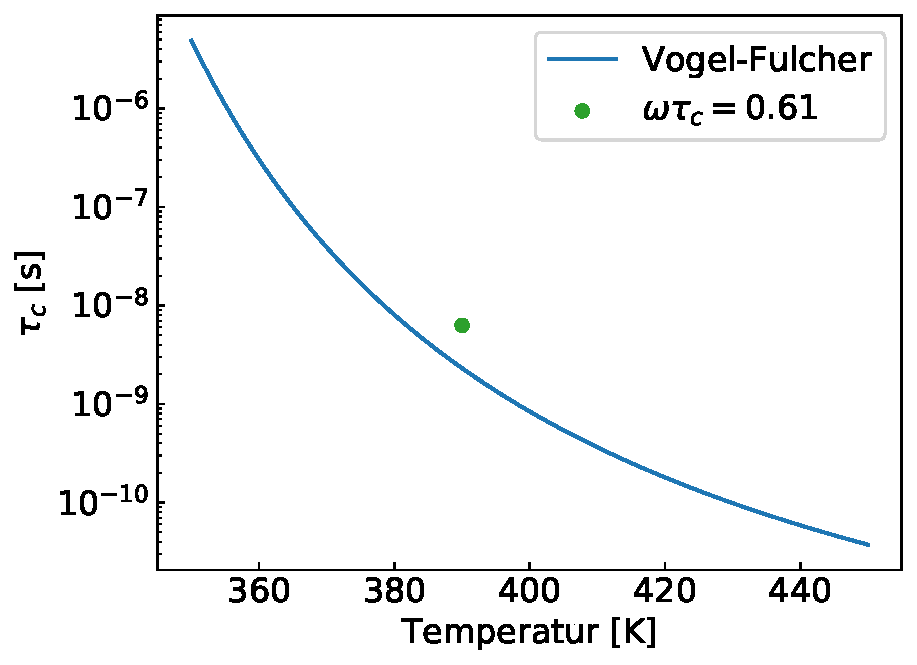
\includegraphics[width=0.49\textwidth]{graphics/zwischenbericht/tau_c_arrhenius_vogel_fulcher.pdf}
  \end{center}
  \vspace{-20pt}
  \caption{Vergleich von Korrelationszeiten basierend auf Vogel-Fulcher-Gesetz \label{fig:korrelationszeiten}}
\end{wrapfigure}
Am $T_1$-Minimum nach Gleichung \eqref{eqn:bpp} gilt $\omega \tau_c \approx \SI{0.61}{}$ \cite[S. 629]{omegatau061}. Das $T_1$-Minimum kann in den Daten bei etwa $T_\text{min} = \SI{390}{K}$ gefunden werden; die Larmorfrequenz liegt bei $\omega_L = \SI{97.1722}{MHz}$, was bedeutet, dass bei $T_\text{min}$ gilt $\tau_c \approx \frac{\SI{0.61}{}}{\omega_L} \approx \SI{6.28}{\nano s}$. Vergleicht man das Vogel-Fulcher-Gesetz mit diesem Punkt, lässt sich erkennen, dass eine gute Übereinstimmung vorliegt.


Die aufgenommenen Daten unterstützen eine biexponentielle Interpretation wie in \eqref{eqn:trans_relax} nur schwerlich, daher wurde lediglich der deutlich zu beobachtende Anteil des Zentralübergangs, $\Delta_c$ und $\omega_c^{(2)}$, für die entsprechenden FWHM- bzw. Schwerpunkts-Daten betrachtet. Für die $T_1$-Daten wird Formel \eqref{eqn:bpp} verwendet. Um einen Ausgangspunkt für die Analyse zu schaffen, wurden alle Fits per Hand erstellt, wobei durch das Ändern der Parameter versucht wurde eine möglichst gute Übereinstimmung zu erreichen.

Für die Spektraldichte $J(\omega)$ kann, wie in Abbildung \ref{fig:triple_vergleich} zu sehen, mit $\eta^2 = 42 - 24 \sqrt{3} \approx \SI{0.43}{}$ \cite{caer} und den Parametern $C_Q = \SI{3e6}{Hz}$ und $\tau_c = \SI{3.9e-14}{s}$ eine vergleichsweise gute Übereinstimmung für die $T_1$-Werte erreicht werden, die Flanken unterscheiden sich jedoch deutlich. Die Abweichungen der FWHM-Werten und der Schwerpunkte sind mit einem Faktor von etwa 4 bzw. etwa 2 bedeutend.
\begin{figure}[htbp]
    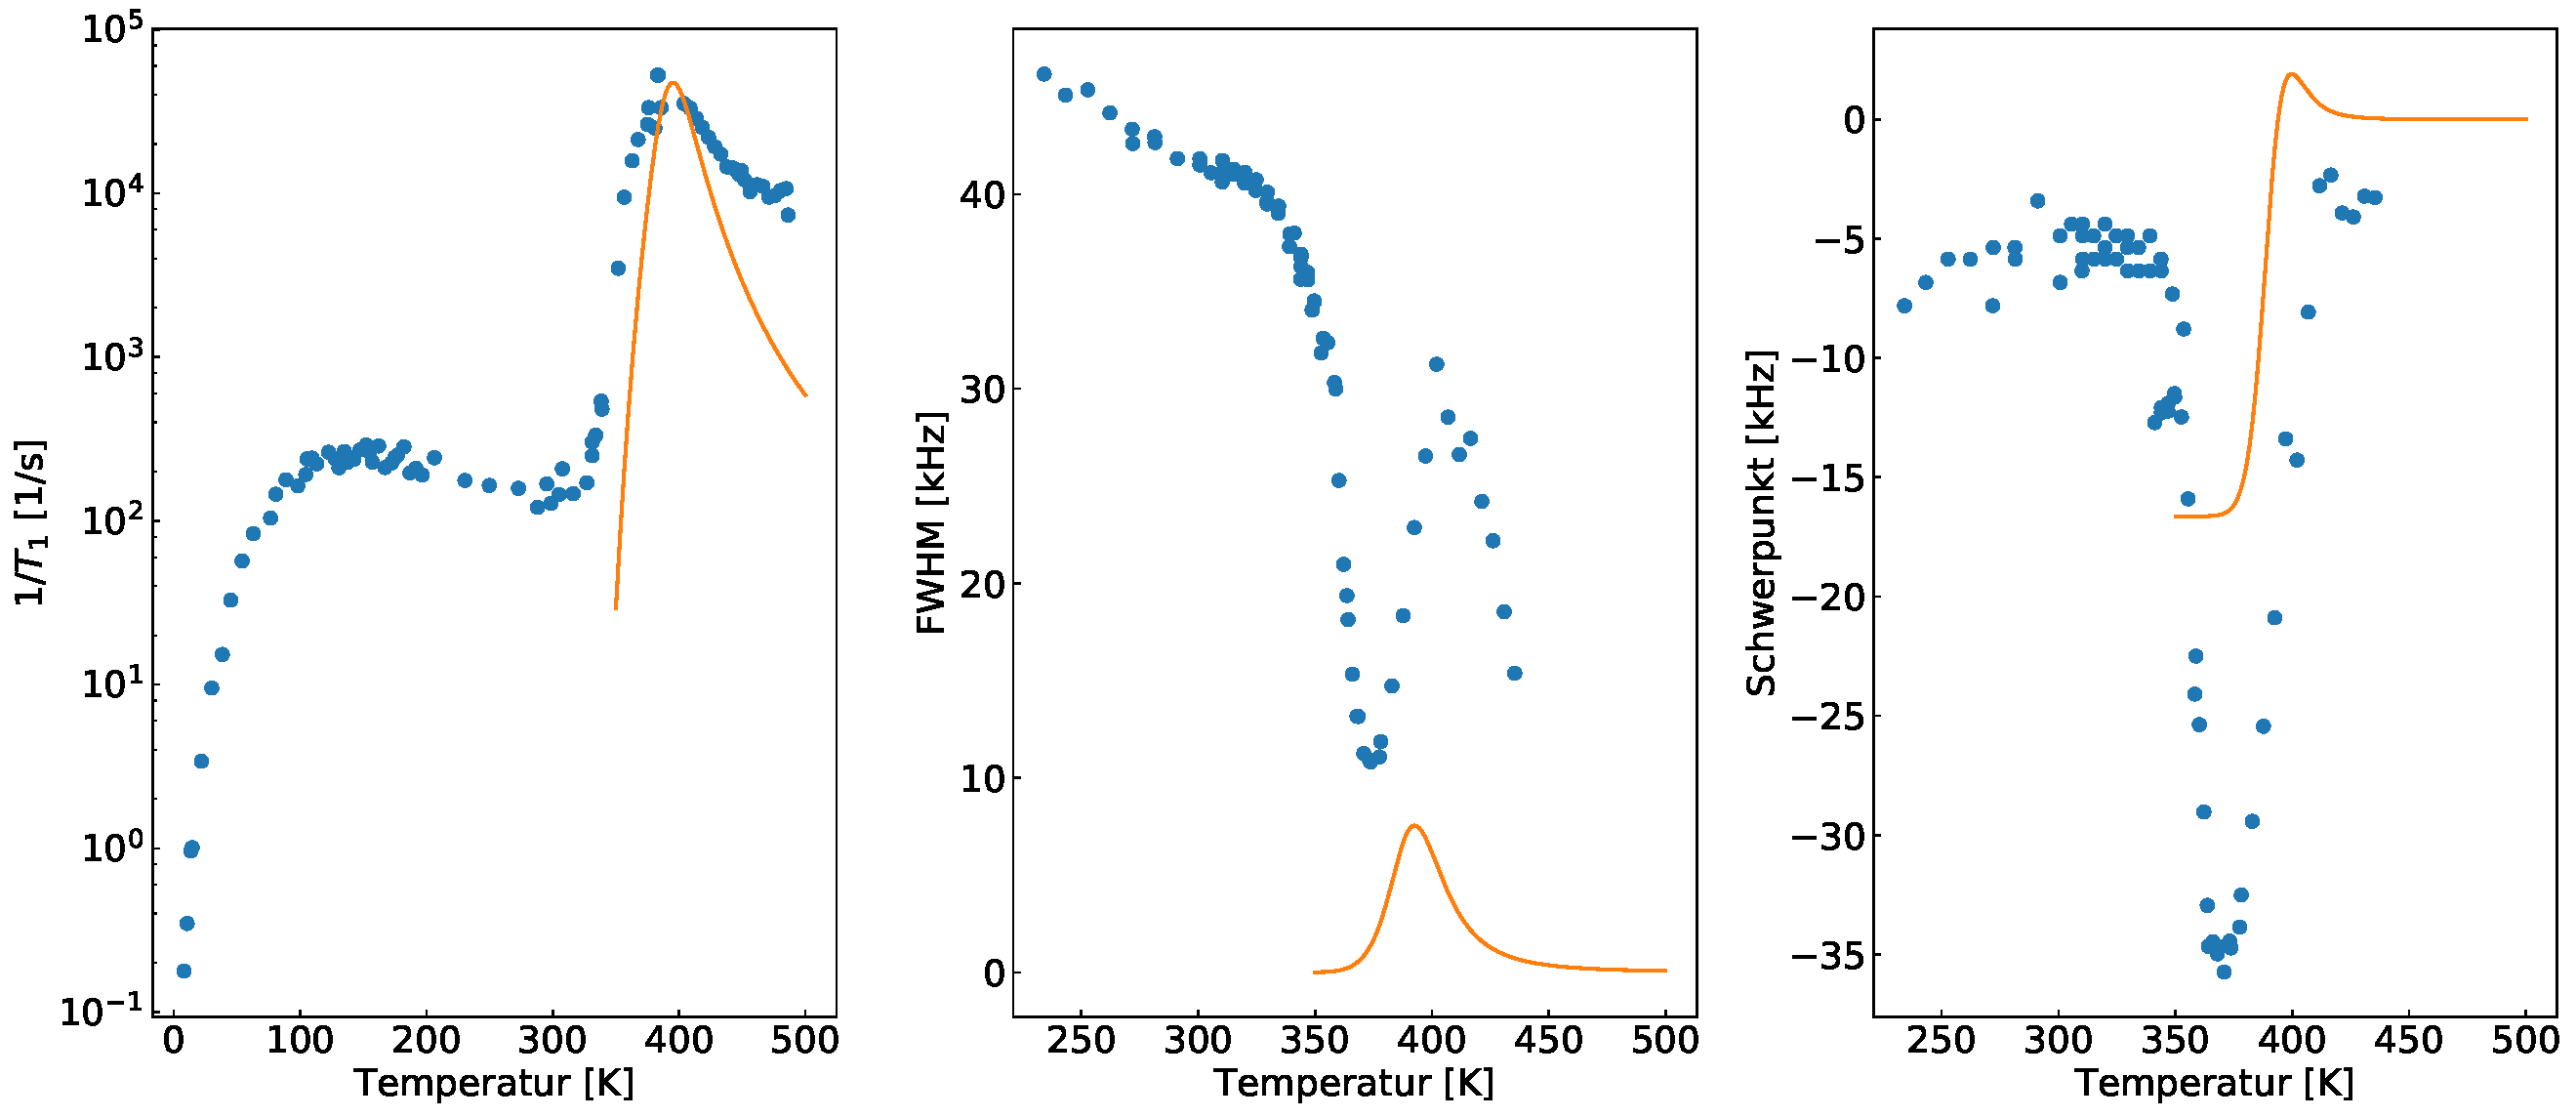
\includegraphics[width=\textwidth]{graphics/zwischenbericht/J_fertig.pdf}
    \caption{Vergleich der $T_1$-, FWHM- und Schwerpunkts-Daten (in blau) und der angepassten Theoriekurven (in orange). \label{fig:triple_vergleich}}
\end{figure}

Eine mögliche Erklärung für die Abweichung der FWHM-Werte könnte sein, dass in diesem Fall nicht, wie nach Formel \eqref{eqn:fwhm}, nur $T_2$, sondern auch das bei Temperaturen um $\SI{400}{K}$ mit etwa $\SI{50}{\micro s}$ äußerst kurze $T_1$ zur Verbreiterung des Spektrums und damit zu dessen FWHM-Werten beiträgt. Erste Versuche, den Effekt der $T_1$-Relaxation aus dem Spektrum herauszurechnen, scheinen vielversprechend. Für die Abweichungen der Schwerpunkts-Daten von der Theorie steht eine entsprechende Erklärung noch aus.

Aus diesem Grund jedoch soll für die Spektraldichten $J_{CC}$ und $J_{CD}$ die FWHM-Werte zunächst nicht betrachtet werden. Gleiches gilt für den Schwerpunkt, da die entsprechenden Imaginärteile der Spektraldichten, $Q_{CC}$ und $Q_{CD}$, nicht zur Verfügung stehen.

Für die Parameter $C_Q = \SI{2.85e6}{Hz}$, $\tau_c = \SI{7e-15}{s}$ und $\alpha = \SI{0.38}{}$ kann mit der Spektraldichte $J_{CC}$ in diesem Temperaturbereich eine noch bessere Übereinstimmung zu den $T_1$-Daten erzielt werden, für die Parameter $C_Q = \SI{2.7e6}{Hz}$, $\tau_c = \SI{4.4e-14}{s}$ und $\gamma = \SI{0.66}{}$ erreicht die Spektraldichte $J_{CD}$ eine leicht bessere Übereinstimmung als die Spektraldichte $J$; die entsprechenden Plots sind in Abbildung \ref{fig:j_cc_j_cd} zu finden.
% \begin{figure}[htbp]
%     \subfigure{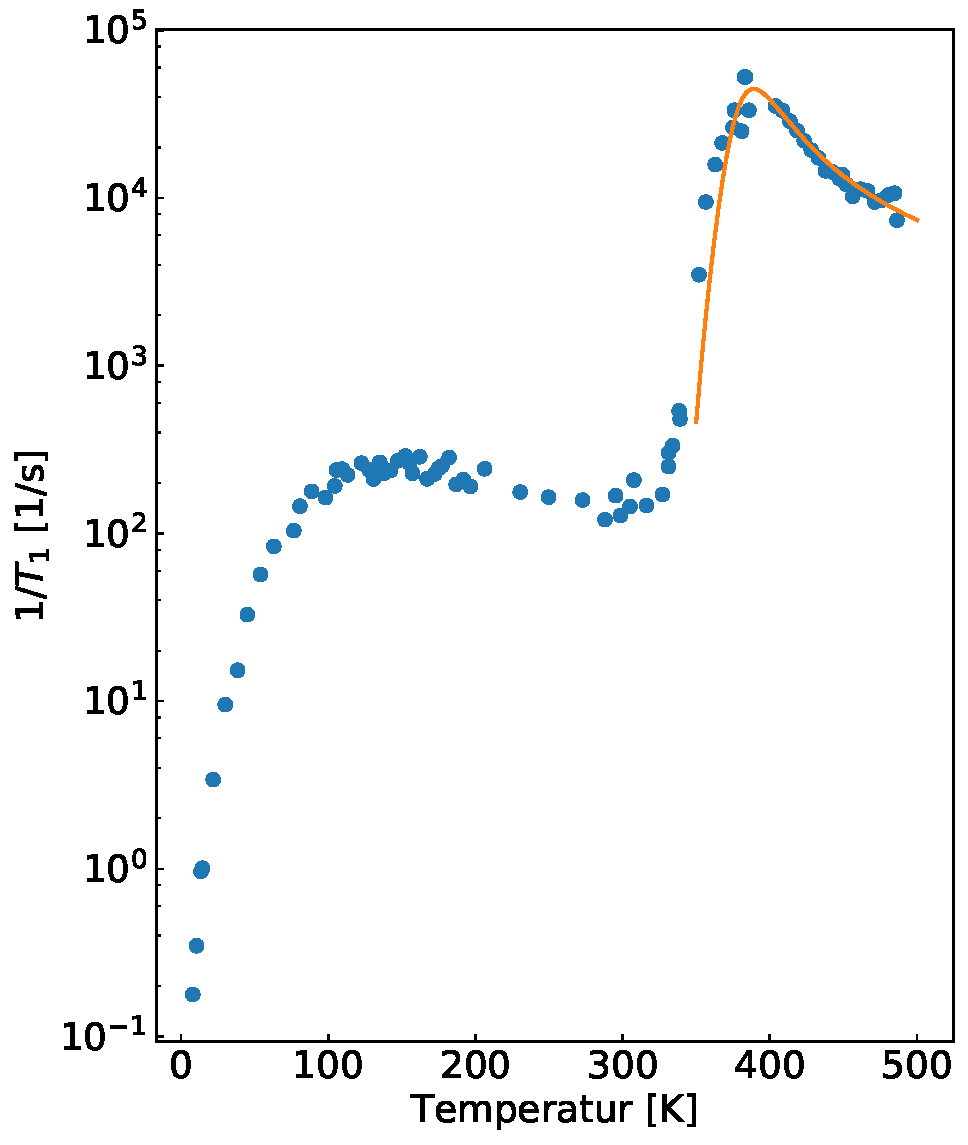
\includegraphics[width=0.49\textwidth]{graphics/zwischenbericht/J_cc.pdf}}\hfill
%     \subfigure{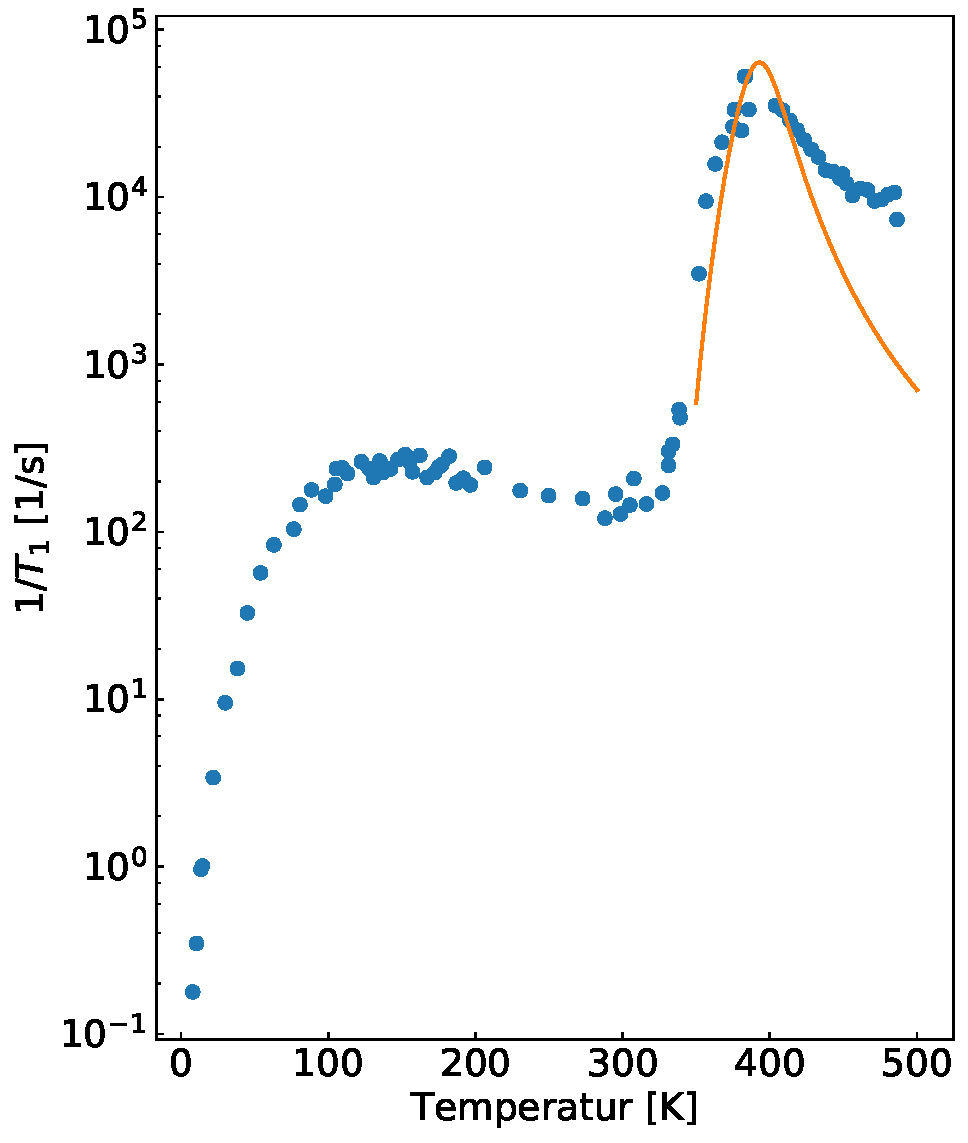
\includegraphics[width=0.49\textwidth]{graphics/zwischenbericht/J_cd.pdf}}
%     \caption{Spektraldichten $J_{CC}$ (links) und $J_{CD}$ (rechts), angepasst an die Daten \label{fig:j_cc_j_cd}}
% \end{figure}
Die nächsten Schritte in dieser Untersuchung sollen darin bestehen, die Auswirkungen der $T_1$-Relaxation auf die Spektrums-Breite zu bestimmen und schlussendlich zu ergründen, ob sich die Messdaten sich mit diesen Theorien zufriedenstellend erklären lassen.





\section{Echos} \label{section:theo:echos}

Um Größen wie $T_1$ und $T_2$ zu messen, werden unterschiedliche Pulsfolgen, also Sequenzen von RF-Pulsen mit bestimmten Längen und Abständen zwischeneinander, ausgenutzt.

Um die longitudinale Relaxation $T_1$ zu messen, wurde folgende Pulsfolge verwendet:
*** Bild
Der erste Puls, ein $\SI{180}{\degree}$-Puls, invertiert die Magnetisierung von $M_\infty$ zu $M_{-\infty}$, wonach diese anfängt zu relaxieren. Da die longitudinale Magnetisierung aufgrund der Spulengeometrie nicht detektierbar ist, muss sie mit $\SI{90}{\degree}$-Puls in die Detektionsebene geklappt werden. Wird dies nach der Evolutionszeit $t_p$ getan, kann also die relaxierende Magnetisierung in Abhängigkeit von $t_p$ bestimmt werden. Der letzte Puls, ein $\SI{180}{\degree}$-Puls, wird Hahn-Echo genannt. Häufig liegen die Momente direkt nach einem Puls in der Totzeit des Detektors, sodass die Magnetisierung faktisch erst gemessen werden kann, wenn sie eine gewisse Zeit abgeklungen ist. Um dieses Problem zu umgehen wird das Hahn-Echo verwendet. 




Nach einer Zeit $\tau_x$ *** nach dem letzten Puls einer Pulsfolge wird die Magnetisierung mit einem $\SI{180}{\degree}$-Puls umgeklappt. Die angesammelten Phasen werden in gleicher Weise subtrahiert, sodass nach der Zeit $2 \tau_x$ *** ein Echo mit maximaler Magnetisierung zu detektieren ist. Das Hahn-Echo kann Teile der Magnetisierung refokussieren, die linear in $I_z$ sind. Dazu zählen zum Beispiel *** und lokale Feldinhomogenitäten. Nicht jedoch wiedergewonnen werden können Teile der Magnetisierung, die durch *** -> T2 verloren wurden. Damit dieser Einfluss bei den Messungen konstant ist, wird in diesem Fall das gleiche $\tau_x$ *** für alle Messungen verwendet.

Es lässt sich so aber offensichtlich mit folgender Pulsfolge $T_2$ bestimmen: Ein $\SI{90}{\degree}$-Puls kippt die Magnetisierung aus dem Gleichgewicht in die Detektionsebene, wo sie sodann anfängt zu dephasieren. Nach der Zeit $\tau_x$ *** wird ein Hahn-Echo durchgeführt und nach $2 \tau_x$ kann die verbliebene Stärke der Magnetisierung gemessen werden. $T_2$ kann so in Abhängigkeit von $\tau_x$ *** aufgenommen werden.

Sowohl an $T_1$- als auch an $T_2$-Daten können Varianten einer Kohlrauschfunktion gefittet werden
*** Formeln
Dabei handelt es sich um Exponentialfunktionen, die mit einem Exponenten $\beta$ gestrecjt werden können. Dieser Exponent erlaubt Abweichungen von der BPP-Theorie, die vin einer einzelnen Korrelationszeit $\tau_c$ ausgeht. ***
